\section{Correlation Quantification}
\label{correlationquantification}
In Section~\ref{matchingresult} we have shown the personal-information-involved password structure distributions and how much does each type of the personal information count in all passwords. These results helped us to draw interesting qualitative conclusions such as users like to use their personal information in their passwords and quantitative conclusions such as birthday appears in 24.63\% passwords, which is the highest percentage among the 6 types of personal information.
However, until this point we do not have a clear idea about how much does personal information correlate to passwords in a quantitative way. Although we have shown useful numbers between each type of personal information and passwords (such as birthday appears in 24.63\% passwords), these numbers are not ideal to describe the passwords because there are many of them. Yet we seek a more comprehensive method to quantify the correlation between passwords and personal information. Thereby we create a new metric -- Coverage -- to quantify the correlation. 

\subsection{Coverage}
\label{coverage}

Coverage is a useful metric to describe how close are personal information and passwords. It is used on every individual user in the dataset. The average Coverage also reflects correlation of the dataset. We will show the computation of coverage and give a detailed example in the following section to illustrate how Coverage works. Besides, we also explain why Coverage is a good metric to describe the correlation between password and all personal information available. 
\subsubsection{Computation Method}
\label{computationmethod}
To compute coverage, we take password and personal information in terms of strings as input. And we use a sliding window approach as in data transmission protocols to compute Coverage. We maintain a dynamic-sized window sliding from the beginning to the end of the password. The initial size of the window is 2. If the segment in the window matched to a certain type of personal information, we enlarge the window by size of 1. Then we try again to match the segment in the window to personal information. If a match is found, we further enlarge the window size until matches no longer exist. At this point we slide the window by one symbol and reset the window size to be the initial size. In the mean time of sliding, we maintain an array of same length as the password. This array is called tag array. Tag array is used to record the length of each matched password segment. For example, a tag array may be [4,4,4,4,0,0,2,2]. This array implies that the first 4 password symbols match certain type of personal information. the 5th and 6th symbols have no match and the last 2 symbols also match certain type of personal information. It does not matter which type do first 4 symbols and last 2 symbols match. When we eventually slide window through the password string thoroughly, the tag array is used to compute the Coverage metric. Coverage is computed as the sum of squares of matched password segment length divided by the square of password length. Mathematically
\begin{equation} \label{eq1}
\begin{split}
CVG & = \sum_{i=1}^n (\frac{l_n^2}{L^2}) \\
\end{split}
\end{equation}
in which $n$ means the number of matched password segment, $l_n$ means the length of corresponding matched password segment, and $L$ means the length of the password. We show the algorithm that is used to compute Coverage in Algorithm~\ref{alg2}. Note that differently from the matching algorithm introduced in Section~\ref{matchingmethod}, we aim to keep the matching for Coverage simpler in order to keep it universally applicable. Namely we try to keep ad-hoc processing on each type of personal information minimum. Toward this end, we do not include various composition of birthday. Cases like DD+MM+YYYY are ignored and we keep only the only case of YYYY+MM+DD, which conforms to Chinese conventions. However, we keep full name and name initials to match names because name initials are very common in Chinese passwords. Besides, only little processing is acceptable in computation of Coverage. As a conclusion, only names have 2 permutations, other personal information keep their original format. A match is found if a password segment is a substring of any of the personal information.


\begin{algorithm}[!]
\caption{Compute Coverage.}
\label{alg2}
\begin{algorithmic}[1]
\Procedure{Cvg}{$pwd$,$infolist$}
\State $windowsize \gets$ 2
\State $pwdlen \gets$ len($pwd$)
\State $matchtag \gets$ [0]*$pwdlen$
\State $matchmark \gets $ 0
\State $cvg \gets $ 0
\While {$windowsize \le $len($pwd$)}
\State $passseg \gets pwd[0:windowsize]$
\If {$passseg$ = substring of $infolist$}
\For {$j \gets matchmark$ to $matchmark$+$windowsize$}
\State $matchtag[j] \gets windowsize$
\EndFor
\If {$windowsize$ != len($pwd$)}
\State $windowsize \gets windowsize$+1
\EndIf
\Else
\State $matchmark \gets matchmark$+$windowsize$
\State $pwd \gets pwd[windowsize:]$
\State $windowsize \gets$ 2
\EndIf
\EndWhile
\For {$eachitem$ in $matchtag$}
\State $cvg \gets cvg + eachitem$
\EndFor
\State \Return $cvg/(pwdlen * pwdlen)$
\EndProcedure
\end{algorithmic}
\end{algorithm}

We illustrate a simple example in Figure~\ref{f1}. In this example, we take a user named Alice, who was born in Aug. 16, 1988. Her password happens to be "alice816". If we apply the algorithm in Section~\ref{matchingresult}, the structure of this password will be [NAME][BD]. Apparently her password is quite related to her personal information. To quantify this relation, we follow Algorithm~\ref{alg2} to compute Coverage for her in each step as shown in Figure~\ref{f1}. (a) The password is prepared for a window to slide through. Note the personal information include "alice" as name and "19880816" as birthday. The tag array is initialized as [0 0 0 0 0 0 0 0]. (b) Window size is initialed to 2 so the first 2 symbols in the password are covered. "al" is a substring of alice's name, so a match is found. Therefore we extend the window size by 1 and the tag array is updated as [2 2 0 0 0 0 0 0]. (c)-(e) Window keeps growing because matches are continuously found. The tag array also keeps updating. (f) The window now covers "alice8", which is not a substring of "alice" or "19880816". Therefore, window size is rest to 2 and tag array remains unchanged. (g) The window of size 2 now covers "81", which is a substring of birthday, again we extend the window by 1 and update tag array to [5 5 5 5 5 2 2 0] (h) After window grows, "816" is also found a match. Tag array is updated to [5 5 5 5 5 3 3 3]. The window does not grow or slide any more because it has reached the end of the password. (i) All symbols have settled. Tag array can now be used to compute Coverage. Based on Equation~\ref{eq1}, the coverage is computed as $CVG  = \sum_{i=1}^2 {{l_n^2} \over {L^2}} = {{5^2 + 3^2}\over{8^2}}= 0.52$.

\begin{figure}[h!]
\centering
  \caption{Coverage - An Example.}{}
  \label{f1}
  \centering
    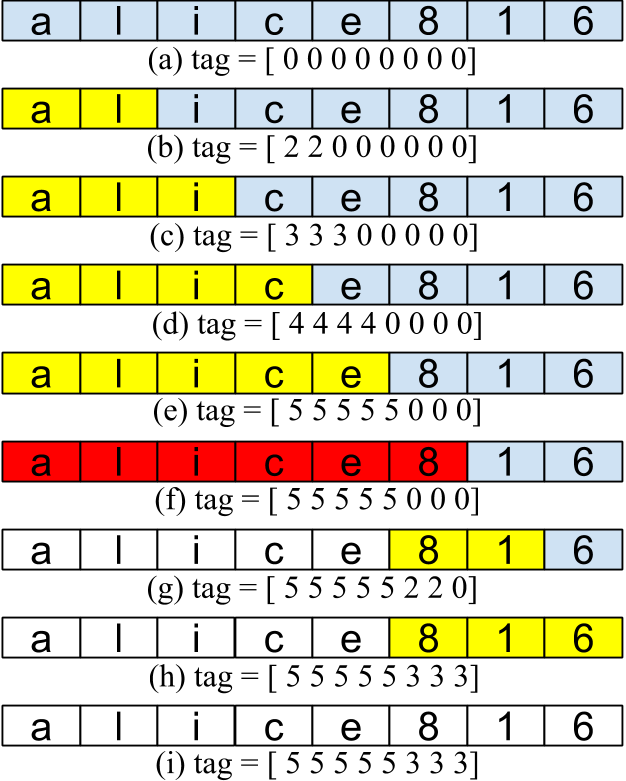
\includegraphics[width=0.3\textwidth]{fig/cvgfig}
\caption*{Grey boxes hold unvisited password symbols. green and red boxes denote that the symbols inside are covered by the sliding window. White boxes denote the symbols inside have been settled (window stops extending). }

\end{figure}


In order to show that Coverage is a useful and reasonable metric, we present 4 features that Coverage has and why we need these features.

\begin{enumerate}[leftmargin=*]
\item By the nature of Equation~\ref{eq1}, Coverage ranges from 0 to 1, in which 0 means no personal information is matched to any password segment and 1 means the entire password is matched to only one type of personal information. 
\item Coverage can be universally applicable for its simplicity. Any kind of personal information can be formatted as a string, check whether or not a password segment is a substring of the string is straightforward. Besides, a few variations of personal information strings may be applied to enhance the completeness and accuracy (like names in our application). Therefore, even certain types of personal information are missing or extra types of personal information are available, Coverage can consistently serve its purpose.
\item Coverage can reflect the length of personal information over the length of password. We need this feature because longer matched password segment naturally indicates stronger correlation. From Equation~\ref{1}, for a matched password segment, the longer the segment is, the larger the numerator will be. It is obvious Coverage measures the correlation strength. \item For personal information segments of same length, Coverage stresses the Continuation of matching. We argue that continuous match is stronger than fragmented match. That is to say, for a given password of length $l$, a matched segment of length $l$ has stronger password than 2 matched segments of length $l_1$ and $l_2$ with $l = l_1 + l_2$. For example, a matched segment of length 6 is expected to have stronger correlation than 2 matched segments of length 2 and 4. We desire this feature because shorter segments usually involve wrong match (coincidence). Since it is very hard to differentiate a real match and a coincidence match, we would like to minimize the effect of wrong matches by taking squares of the matched segments to compute the Coverage.
\end{enumerate}

\subsection{Result}
We apply Algorithm~\ref{alg2} on every user of 12306 dataset. The result is shown as a cumulative distribution graph in Figure~\ref{f2}. From the figure we have the following observation
\begin{enumerate}[leftmargin=*]
\item Half of the users have Coverage higher than 0.186, implying that  a significant portion of user passwords have relatively high correlation to their personal information.
\item 9.9\% users have 0 Coverage. 0 Coverage indicates there is no possible correlation between the users' passwords and their personal information.
\item 10.5\% users have Coverage of 1, which means that 11.9\% passwords are perfectly matched to exactly one type of personal information. However, Only 13.4\% users have Coverage higher than 0.5 and lower than 1.0. 
\end{enumerate}

\begin{figure}[h!]
\centering
  \caption{Coverage distribution - 12306.}{}
  \label{f2}
  \centering
    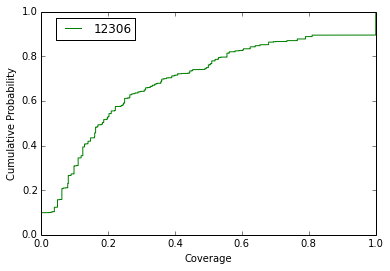
\includegraphics[width=0.45\textwidth]{fig/cvghist}
\end{figure}

Besides, the average Coverage for 12306 dataset is 0.309. We also compute the average Coverages for male and female groups that are used in Section~\ref{genderdifference}, in which we concluded that male users are more likely to include personal information in their passwords. It turns out that the average Coverage for male group is 0.314 and the average Coverage for female group is 0.269. Our result indicates that the correlation between password and personal information for male users is higher. It complies with our previous conclusion. Therefore, it shows that Coverage works well to determine the correlation between passwords and personal information.

\subsection{Coverage Usage}
Coverage can be used in many scenarios. Firstly, it can be used as a reserach metric to describe a dataset. Coverage directly reflects the correlation between password and available personal information. Investigating how users from different systems behave regarding to constructing their passwords using personal information would be an interesting future work. 

Apparently, Coverage would be very useful in password strength meters. Strength meters are reported as mostly ad-hoc \cite{de2014very}. Most meters dumbly give score based on password structures and length, or blacklist commonly used passwords (such as "password"). There are also meters that do simple social profile analysis such as passwords cannot have the users' names or passwords cannot be the same as account names. However, these simple analysis mechanisms can be easily fooled by mangling the password a little. In cases of password strength meters, Coverage is able to cover the unnoticed corner of personal information. Consider the routine for creating an account. Users usually fill in some profile information such as name, birthday, email address, etc and create a password. At this moment password meters will offer feedback of password strength normally in bar forms. Since personal information is available, it is straightforward to set Coverage as part of strength measurement. Apparently, higher Coverage indicates vulnerable passwords. Systems can even ban passwords when they surpass a preset Coverage threshold. Additionally, users cannot easily escape Coverage measurement by simple mangling, thus their passwords are further secured. 

Coverage can also be added to existing tools to enhance their capabilities. There are several Markov Model based tools that predict the next character when the user creates a password \cite{komanduri2014telepathwords}\cite{weir2010testing}. Users would be surprised to find that the next character in their mind matches exactly the tool output and then switch to a more unpredictable passwords. Coverage is able to work in these tools as an enhancement -- When Coverage is rather high, it is easy to predict what the next character of user input is.

